\documentclass[portfolio.tex]{subfiles}
\begin{document}
	\Chapter{Week 1}{The Basics of Web Development}
		\section{Introduction}
			Web development requires the use of three languages: HTML, CSS and Javascript. These three languages work together to tell the browser how a website should \underline{\textbf{look}} and \underline{\textbf{act}}. By understanding them thoroughly, we are able to create high quality, responsive websites, that users will find visually pleasing and easy to use.\\
		\section{Weekly Content}
			\subsection{HTML}
				\subsubsection{Introduction to HTML}

					Hyper Text Markup Language is a structured way to store the information which will be displayed on a webpage. More simply, HTML tells the browser \textbf{WHAT} to display.\\
					\\
					 HTML uses tags to hold the data. An example of a tag is: $\color{blue}<body>\color{red}</body>$. The opening tag in blue, has a matching closing tag in red.  Relevant information is placed between the two tags. For our body example earlier, the browser will know that the information for the body will be between the opening body tag and the closing body tag.\\

					 Attributes for tags can be set within the opening tag. An example of using attributes to assign a class to a p element would look like: $<$p \textbf{class="text"}$>$.  A class groups a number of elements together, while another attribute \textbf{id} refers to only one element. There are many other HTML attributes to help us configure our elements. For a large list of possible attributes. visit \seqsplit{https://www.w3schools.com/tags/ref\_attributes.asp}.\\



				\subsubsection{Boilerplate To Get Started}
				\label{html-boiler}
				To get started writing an HTML document, there is some boilerplate code that must \textit{almost} always be present:\\

					\begin{lstlisting}
<!DOCTYPE html>
<html>
	<head>
		<title>Title</title>
		<script src="INSERT LINK TO JAVASCRIPT FILE HERE"></script>
		<link rel="stylesheet" type="text/css" href="INSERT LINK TO CSS FILE HERE">
	</head>
		<body>
			INSERT HTML TO DISPLAY HERE.
		</body>
</html>
					\end{lstlisting}

						\vspace{0.5cm}
						\textbf{Notice the indentation!} To make this code easier to read, any tag that is inside another tag will be indented further. For example, it is easy to see that the head tag is inside the html tag. See the below table for descriptions of each tag.\\

					{\centering
						\begin{tabular}{P{4cm}p{11cm}}
						\toprule
						\large\textbf{Tag} & \large\textbf{Description}\\
						\toprule
						$<$!DOCTYPE$>$ & This is to let the browser know that this is a current HTML5 document. Previous versions of html will have different codes to insert here. \autocite{doctype} \\
						\hline
						$<$html$>$...$<$/html$>$ &  This is the html document, all information will be inside this tag\\
						\hline
						$<$head$>$...$<$/head$>$ &  This contains information that will not be displayed within the webpage itself.\\
						\hline
						$<$title$>$...$<$/title$>$ &  The title to the webpage. This will be displayed either in the browser's title bar area at the top of the window, or the tab area.\\
						\hline
						$<$script$>$...$<$/script$>$ & This can either contain JavaScript code directly, or have a src attribute that links to an external file (either locally, or from a http link) \\
						\hline
						$<$link$>$& This  links to some exterior document. The most common use of the link tag is to link to an external css file, but other documents that might be linked are icons, and licenses. \autocite{w3-link} \\
						\hline
						$<$body$>$& Body contains all the information that will be displayed on the website itself. \\
						\bottomrule
					\end{tabular}
				}

				\subsubsection{Other useful tags and descriptions}
					\begin{itemize}
						\item $<$\textbf{p}$>$...$<$\textbf{/p}$>$ contains a paragraph of text.
						\item $<$\textbf{h\#}$>$...$<$\textbf{/h\#}$>$ contains a header. \# is replaced by the size of header, 1 is the largest and 6 is the smallest.
						\item $<$\textbf{div}$>$...$<$\textbf{/div}$>$ is a generic tag that creates a container for other elements.
						\item $<$\textbf{a href="..."}$>$...$<$\textbf{/a}$>$ creates a hyperlink to another page. href is the link, and the text between the tags is displayed to the user.
				\end{itemize}
				\subsubsection{\textbf{Tags without closing tags}}

						There are a few tags which don't require a closing tag. These tags get information through other means, like the $<$img /$>$ tag, which knows what image to render using the \textbf{src} attribute.
					\begin{itemize}
						\item $<$\textbf{img src="image location"}$>$ loads an image from either a website, or local storage.

					\end{itemize}

				\vspace{0.5cm}
				\subsubsection{Tables}


				Tables are a great way to organise information on a website. They act the same way as tables within commonly used word processors such as Microsoft Word with columns and rows. \\

				The table is broken into two parts: $<$thead$>$ which uses $<$th$>$ to create header cells, and $<$tbody$>$ which uses $<$td$>$ to create regular cells. The graphic below provides a clear understanding of the structure of a table. Remember, the values for each cell are placed in the inner most tags (th and td).\\

				\begin{center}
					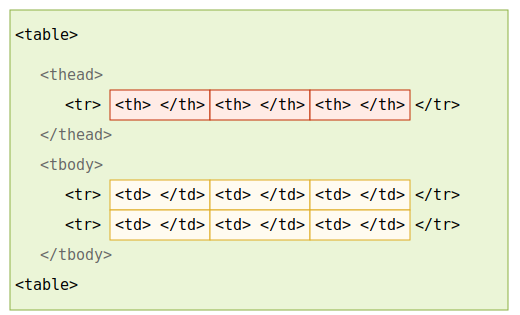
\includegraphics[width=0.9\linewidth]{html-table.png} \\
					\autocite{html-table}\\
				\end{center}




				\subsubsection{Forms}
					Forms are a collection of input fields within HTML. The user can enter different types of information depending on the type of input field. When the form is submitted, the browser will collect all the inputs and either send them to a url (if the attribute \textbf{action} is present on the form), or will send them to a JavaScript function (if the attribute \textbf{onsubmit} is present). An example of a form with the inputs name, age and location might be: \label{form-html} \\
					\vspace{1cm}
					\begin{lstlisting}
<form onsubmit="submitForm(event)">
	<label for="name">Name</label>
	<input type="text" id="name" size=20 maxlength=20>
	<label for="age">Age</label>
	<input type="number" id="age" max=120>
	<label for="location">Location</label>
	<input type="text" id="location">
	<input class="button" type="submit" value="Submit">
	<input class="button" type="reset" value="Cancel">
</form>

					\end{lstlisting}
				\vspace{1cm}
					Which would output:\\

				\begin{center}
					\includegraphics[width=14cm]{html-form.png}
				\end{center}

			\hspace{-1.5cm}
			\begin{tabular}{l l}
				\begin{minipage}{0.5\textwidth}
					\includegraphics[trim=0 0 0 80, clip, width=0.9\linewidth]{email_address_invalid.png} 
\\

				\end{minipage}
				&
				\begin{minipage}{0.5\textwidth}
					\subsubsection{Inputs}
					In HTML5, inputs can have a variety of types (To name a few: text, number, email). Some inputs limit what can be inputted into the field, such as an input with the type email will only accept properly formatted emails. \\
				\end{minipage}
			\end{tabular}

			\hspace{-0.7cm}

			\splitpage{
				Another reason to use proper input types is to create a responsive website, where a different keyboard will appear on a mobile device depending on the input type. For example, an input with the type numbers will bring up a keyboard on mobile devices that only includes numbers. See an an example of this below:\\

				Input fields can also be displayed as buttons, for example if the input type is submit or reset as seen in the example form above.\\

				For accessibility reasons, each input must be accompanied by a label tag, which uses the \textbf{for} attribute to connect to an input's id.
			}{
				\centering
				\includegraphics[width=0.8\linewidth]{number-keyboard-example.png}
			}


			\vspace{1cm}
			\subsection{CSS}
			\vspace{0.5cm}
			\splitpage{
				\centering
				\includegraphics[width=0.8\linewidth]{no-css-example.png}\\
			}
			{
				\subsubsection{Introduction to CSS}
					Cascading Style Sheets tells the browser \textbf{HOW} to display the information in the HTML file. Without CSS the default styling is used, which means the webpage doesn't look very good, and will bore the user. This is why we use CSS!\\


				\subsubsection{Basic Syntax}
					CSS uses property name and value pairs separated by a colon. Different pairs are separated by a semi-colon. An example of making the text of an element blue would be: "\textbf{{\color{red}color}: {\color{blue}blue};}" where color is the \underline{property name}(red) and blue is the \underline{property value}(blue).\\


			}

			\vspace{0.5cm}
				Specifying the elements for these styles to be applied is done using some of the following options: \\


					\vspace{0.5cm}
					{\centering
						\begin{tabular}{P{4cm}p{11cm}}
							\toprule[1.5pt]
							\textbf{tag} & This will apply a style to every element of a particular tag. For example, if p is used, every paragraph tag will have the specified styles applied. Note the lack of punctuation before the tag. \\
							\midrule
							\textbf{.class} &  This will apply styles to every element with a particular class. A class is specified with a period before the class name. \\
							\midrule
							\textbf{\#id} &  This will apply styles to the element with a particular id. An id is specified with a hashtag before the id name. \\
							\bottomrule[1.5pt]
						\end{tabular}
					}

					\vspace{0.8cm}

					In the following example, every element with the class "specific-class" would have a margin of 10 pixels and a border that is 1 pixel thick, solid and black.\\

					\vspace{0.2cm}
					\begin{lstlisting}
.specific-class {
	margin: 10px;
	border: 1px solid black;
}
					\end{lstlisting}
					\vspace{0.2cm}

				\subsubsection{Location of CSS}
					There are three options for where to place CSS code:\\

					\begin{enumerate}
						\item \textbf{Inline}
							Placed within the html code within the element. Example: $<$p style="color: red;"$>$
						\item \textbf{Internal}
							Placed within the style tag, usually within the head tag. Example:  $<$style$>$p \{ color: red;\}$<$style$>$
						\item \textbf{External}
							Placed within an external .css file. This is then linked via the link tag as seen in \ref{html-boiler}.
					\end{enumerate}

					This also effects how certain elements will override others. For example, any inline style will override any internal or external style, and any internal style will override any external style. The code is also read top to bottom, so styles at the bottom will override styles at the top.

				\subsubsection{CSS Box}

					\begin{center}
						\includegraphics[width=0.8\linewidth]{"CSS box.png"}\\
						\autocite{w3-box}\\
					\end{center}

					Every element on a webpage is contained in the box above. The outer most layer, margin, is the space outside the border. This will change the perception of how far away the box is from other boxes. After the margins and border, is the padding, this is the space between the border and the content. Good use of the CSS box is critical to creating good spacing within a webpage.

			\subsection{JavaScript}
				\label{week-1-js}
				\bigskip
				\subsubsection{Introduction to Javascript}
					JavaScript is a scripting language that is commonly used in web browsers. It has expanded outside of its original purpose to be able to do much more with the help of other programs such as NodeJS.\\

				\subsubsection{Declaring Variables}
					There are two options when declaring variables depending on if it is mutable or not. If the variable cannot be modified after initialization, use the keyword \textbf{const} followed by the variable name. For example \textbf{const number = 2}. If the variable is mutable, then use the keyword \textbf{let}. An example for this would be \textbf{let letter = 'L'}, where letter can be modified at a later time.
				\subsubsection{Declaring and Calling Functions}
					To declare a function, first use the function keyword, followed by the name, and a list of parameters within parenthesis. The internal code of the function is then placed within curly braces. To return a value to the calling function, simply use the keyword \textbf{return}. Example:\\

					\begin{lstlisting}
function addTwoNumbers(num1, num2) {
	return num1 + num2;
}
					\end{lstlisting}
					\vspace{0.5cm}

					Then to call this function, use \textbf{addTwoNumbers(230, 384)}. Functions allow us to reuse code, instead of rewriting it every time.

				\subsubsection{Window and Document Objects}
					Two useful objects within JavaScript is the window and document objects. \\

					The window object references the entire browser window. This allows access to properties such as  the location, history, height, width, etc. \\

					The document object is a child of the window object. This contains everything that is displayed on the website. This includes the HTML and CSS. There are document methods that allow you to get an element by its id ( \textbf{getElementById()} ), as well as by its class ( \textbf{ getElementsByClass()}  ), and many more. For a full list of methods available within Document, see \\ \seqsplit{https://developer.mozilla.org/en-US/docs/Web/API/Document}\\


				\subsubsection{More JavaScript}
					JavaScript is covered in much greater detail in Week 3. See \ref{week-3-js}.\\

			\subsection{Vue.js}
				\subsubsection{Introduction to Vue}
					Vue.js is a framework that allows the creation of responsive user interfaces while reducing the amount of code actually written. It works with HTML/CSS/JavaScript to provide re-usable components, templates, state handling, and much more. \autocite{vue}\\

				\subsubsection{Templates}
					Within Vue, templates can be created. These templates contain the information displayed on the website, similar to HTML. In fact all HTML will work within these templates, but the templates include extra features to make responsive design much easier.  \\

					Templates allow for a reduction in code compared to traditional HTML. By finding common \textit{structures} within the HTML, templates can be created so that different data can be inserted into these reusable structures. This means that we don't have to spend time re-writing the same structures over and over. Syntactically, Vue uses double curly braces to represent areas where data will be inserted later. \textbf{\{\{ name \}\}} will be replaced with the value of the name variable.\\ \autocite{vue-template}\\

					For a simple example of where templating can reduce the amount of code written, refer back to \ref{html-boiler}. Each html document you create has to have these pieces of code. Instead of rewriting this every time,  a template could be created as follows:\\

					\begin{lstlisting}
<html>
	<head>
		<title>Title</title>
		<script src="{{ jsFile}}"></script>
		<link rel="stylesheet" type="text/css" href="cssFile">
	</head>
	<body>
		<h1>{{ title }}</h1>
		<p> {{ paragraph }}
	</body>
</html>
					\end{lstlisting}

					\vspace{0.5cm}

					This could then be reused for many different websites with different information by supplying different values for the variables title, paragraph, jsFile, etc.. This of course can be expanded to much more complicated websites where there are many of the same pages. Consider Facebook, where everyone has their own profile page. These pages are standardised across the website to look the same, but the information is different on each one. A template is made once, then whenever the page is rendered it is filled with the appropriate data.\\

					 This then becomes even more powerful when responsive web apps are considered. If required, different templates could be created for each style of device (small mobile, tablet, desktop) to create a very different experience. When the user visits the web app, the appropriate template will be selected and used, all while the data remains the same.\\


					\subsubsection{Components}
						Components are re-usable snippets of code that abstract away some code. Pre-defined options(or "props") can also be passed to the components to affect what is rendered making them much more flexible. Many components can then be built together to form much larger components, and then those components combined to create a whole application. All while using minimal code compared to pure HTML/CSS/JS. \\

				\hspace{-0.8cm}
				\splitpage{
					In this small example, the link component and the button component are reused within two separate, larger components. This is incredibly small compared to many web apps, which would reuse the components many, many times. This reduces repetition of code. \autocite{vue-component}
				}{
					\includegraphics[width=0.9\linewidth]{component-app.png}
}


		\section{Practical Tasks}
			\subsection{1 - HTML}
				 This task provided a very basic example to help learn the bare bones of HTML, and its commonly used tags. It also allowed practice in creating both a table and input form.
				\subsubsection{Code}
				The code can be viewed at \seqsplit{https://github.com/BrandonMurch/SIT120/blob/021a2694432d61e32c9fba191ee7579c2dfdb955/Practical\%20Tasks/Practical\%201/task1.html}


				\subsubsection{Screenshot}
					\label{task-1.1}
					\includegraphics[trim=10 0 0 10, clip, width=\linewidth]{"Task 1 Evidence.png"}



			\subsection{2 - CSS}
				This task focussed on introducing CSS, which makes the website look attractive. It allows practice with the structure of CSS, as well as with properties that are commonly used.\\

				Building upon the last task, I formatted the website using CSS. This allowed me to create a  website that has two columns. One which contains the table of entries, the other that contains the form to input new entries. The image at the top of the page is then modified to look slimmer and stretch the width of the window, while the title is centred below. \\

				Using a two-column design used the space much more intelligently than the default styling, which would have spread both the table, and form across the entire screen, using double the vertical space.\\

				\subsubsection{Code}
				See code on \seqsplit{https://github.com/BrandonMurch/SIT120/blob/021a2694432d61e32c9fba191ee7579c2dfdb955/Practical\%20Tasks/Practical\%201/task2.css}


				\subsubsection{Screenshot}
					See \ref{task-1.1} since these tasks are combined into one website.\\

				\subsubsection{Useful Code}
					There are many ways to centre an element in CSS, this (\ref{css-center-element}) is a pretty simple and useful one which can either centre an element horizontally, vertically or both. This doesn't rely on any of the more advanced CSS features such as flexbox or grid.\\

			\subsection{3 - JavaScript}
				I made a small JavaScript function that takes the inputs within the form, and dynamically updates the table. I also created a separate website to calculate the inputted student scores. This helped practice modifying the DOM dynamically with JavaScript, which allows for a seamless experience as the user, since information or elements can be modified without refreshing the page. This helps us to understand on a simple level, how frameworks such as Vue work under the hood. \\

				\subsubsection{Code}
					See code for the input form: \\

					\seqsplit{https://github.com/BrandonMurch/SIT120/blob/021a2694432d61e32c9fba191ee7579c2dfdb955/Practical\%20Tasks/Practical\%201/task3.js}\\

					and for the student grades: \\

					\seqsplit{https://github.com/BrandonMurch/SIT120/tree/main/Practical\%20Tasks/Practical\%201/task3\%20-\%20student\%20grades}

				\subsubsection{Useful Code}
					Being able to round numbers in JavaScript was useful in this project, since otherwise there could be tens of decimal places. To accomplish this I used variable.toFixed() [\ref{js-round-number}]

				\subsubsection{Screenshot}
					\textbf{Before form submission:} \\
					\includegraphics[width=\linewidth]{"Task 3 Before.png"}
					\textbf{After form submission:}\\
					\includegraphics[width=\linewidth]{"Task 3 After.png"}\\

					\hspace{-0.8cm}
					\splitpage{
						\textbf{Before score calculation:} \\
						\includegraphics[width=0.9\textwidth]{"scores empty.png"}\\
					}{
						\textbf{After score calculation:}\\
						\includegraphics[width=0.9\textwidth]{"scores calculated.png"}\\
					}


			\subsection{4 - Vue.js}
				A small Todo app with three default items of a classic grocery list. New tasks can be added through the input text box. Tasks can be clicked to complete them. \\

				This task introduced the concept of components. The component $<$todo-item$>$ was reused multiple times, reinforcing the utility of components. From this it shows if they are this beneficial in smaller applications, they must be exponentially so in large applications, making them incredibly important to understand for web developers.\\

				\subsubsection{Code}
				See the code on \seqsplit{https://github.com/BrandonMurch/SIT120/tree/main/Practical\%201/task4}.

				\subsubsection{Useful Code}
					I found Window.onLoad() [\ref{js-window-onload}] to be useful in ensuring the entire page is loaded before Vue tries to reference an element. Otherwise there were errors when placing scripts at the beginning of the HTML file. The script would load before the HTML, and Vue would not be able to find the element to attach itself to.\\
				\subsubsection{Screenshot}
					\begin{center}
						\includegraphics[width=8cm]{"Vue Todo.png"}
					\end{center}

		\section{Project}
			\subsection{What I completed this week}
				This week I have read through the \textbf{Assignment 1: Guidelines and Rubrics}. I have understood what is required of the assignment, and started to make notes of ideas/requirements that will help me to complete this assignment.
			\subsection{What I will complete next week}
				Next week I will do research and think of an idea for my project. I expect this to take a fair bit of time to find a good idea that can be original, as well as managed within the time limitations of the course. This should take me approx. 4 hours.

	\pagebreak

\end{document}